\section{Lecture 6}
\subsection{Clarification on BIBO Stability}
\begin{itemize}
	\item When we say a "bounded" signal, we mean that the amplitude of the signal is bounded at all times:
		\[
		|x(t)| < \infty \ \forall t \in \R
		\] 
		The same definition follows for discrete-time signals. 
	\item For LTI systems, we call the system BIBO stable if and only if its impulse \( h(t) \) is absolutely 
		integrable:
		\[
		\int_{-\infty}^{\infty} |h(t)| \diff t < \infty
		\] 
\end{itemize}
\subsection{Cross-Correlation}
\begin{itemize}
	\item The cross correlation between two signals \( r_{xy}(t) = r_{yx}(-t) \). To show this explicitly, we 
		look at the cross-correlation equation:
		\begin{align*}
			r_{xy}(t) &= \int_{-\infty}^{\infty} x(\tau)y(t + \tau) \diff \tau \\
			r_{yx}(t) &= \int_{-\infty}^{\infty} y(\tau) x(t + \tau) \diff \tau  
	\end{align*} 
	But for the second equation, we can define a \( \tau' = t + \tau\), so then we get: 
	\[
	r_{yx}(t) = \int_{-\infty}^{\infty} y(\tau' - t)x(\tau') \diff \tau' = \int_{-\infty}^{\infty} 
	x(\tau') y(-t + \tau') \diff \tau'
	\] 
	This looks like the first equation except we have \( -t \) instead of \( t \). Therefore, we have 
	\( r_{xy}(t) = r_{yx}(-t) \). The same works for discrete time: \( r_{xy}[n] = r_{yx}[-n] \). 
\end{itemize}

\subsection{More Convolution Properties} 
\begin{itemize}
	\item \textbf{Differentiation property:} Given \( y(t) = x(t) * h(t) \), then:
		\[
			\dv{t} y(t) = x(t) * \dv{h(t)}{t} = \dv{x(t)}{t} * h(t)
		\] 
	\item \textbf{Intergration Property:} Given \( y(t) = x(t) * h(t) \), we have:
		\[
		\int_{-\infty}^{t'} y(t) \diff  t = x(t) * \int_{-\infty}^{t'} h(\tau)\diff \tau 
		\] 
\end{itemize}
\subsection{Fourier Transform} 
\begin{itemize}
	\item Recall the frequency response of an LTI system:
		\begin{center}
			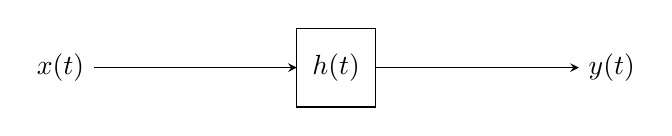
\begin{tikzpicture}
				\node (A) at (-3, 0) {\( x(t) \) };
				\node (B) at (4, 0) {\( y(t) \) };
				\draw[-stealth] (A) -- (0, 0);
				\draw (0, -0.5) rectangle node {\( h(t) \) } (1, 0.5);
				\draw[-stealth] (1, 0) -- (B);
			\end{tikzpicture}
		\end{center}
		Recall that we can characterize \( y(t) \) via a convolution: 
		\[
		y(t) = \int_{-\infty}^{\infty} x(\tau) h(t - \tau) \diff  \tau 
		\] 
	\item Recall that the harmonic response of an LTI system is given by \( H(\omega) e^{j \omega t} \), where 
		\begin{align*}
			H(f) &\equiv \int e^{j 2\pi f t}h(t) \diff  t\\
			H(\omega) &\equiv \int e^{i \omega t} h(t) \diff t
		\end{align*}
	\item The Fourier transform is defined as:
		\[
		H(f) \equiv \mathcal F \{h(t)\} \equiv \int_{-\infty}^{\infty} h(t) e^{-j 2\pi ft }\diff  t 
		\] 
		This transforms the signal \( h(t)  \) from the time domain into the frequency domain.   
	\item The inverse Fourier transform is:
		\[
			h(t) = \mathcal F^{-1} \{H(f)\} = \int_{-\infty}^{\infty} H(f) e^{j 2\pi ft}\diff  f 
		\] 
	\item We can also write this in terms of \( \omega \) :
		\begin{align*}
			H(\omega) &= \mathcal F \{h(t)\} = \int_{-\infty}^{\infty} h(t) e^{-j \omega t} \diff t \\
			h(t) &= \mathcal F^{-1}\{H(\omega)\} = \frac{1}{2\pi}\int_{-\infty}^{\infty} H(\omega) e^{j \omega t}
			\diff \omega\\
	\end{align*}
	The factor of \( \frac{1}{2\pi} \) that exists in the IFT for \( \omega \) is a result of the fact that we have 
	\( \omega = 2\pi f \).
\end{itemize}
